\documentclass[12pt]{article}

\usepackage{sbc-template}
\usepackage{graphicx,url}
\usepackage[utf8]{inputenc}
\usepackage[brazil]{babel}
\usepackage{booktabs}
\usepackage{multirow}
\usepackage{float}
\usepackage{amsmath}

\sloppy

\title{Análise Estatística de Métricas de Código-Fonte\\do Framework Neo4j}

\author{Igor Mariano Lopes Rodrigues\inst{1}, Filipe Oliveira de Saldanha da Gama\inst{1}}

\address{IBMEC -- Curso de Graduação em Engenharia de Software\\
  \email{\{202407095992,202303161085\}@alunos.ibmec.edu.br}
}

\begin{document}

\maketitle

\begin{abstract}
This paper presents a statistical analysis of source code metrics from the Neo4j framework using the GitHub Bug Dataset v1.1, covering class-level (7{,}917 instances) and file-level (4{,}261 instances) granularities. Descriptive statistics, normality tests (Shapiro-Wilk and Lilliefors), Pearson and Spearman correlations, multicollinearity analysis (VIF), and cost-sensitive logistic regression with LOOCV validation were applied. Strong correlations among size and complexity metrics were found (e.g., LOC$\times$LLOC: $r = 0.99$). All distributions are non-normal, and a severe class imbalance ($<0.15\%$ positive) fundamentally limits predictive modeling---with only 8 and 6 bug instances, the Events Per Variable ratio is far below the recommended minimum of 10, rendering any classifier unreliable.
\end{abstract}

\begin{resumo}
Este artigo apresenta uma análise estatística de métricas de código-fonte do framework Neo4j, utilizando o GitHub Bug Dataset v1.1, abrangendo os níveis classe (7.917 instâncias) e arquivo (4.261 instâncias). Foram aplicados estatística descritiva, testes de normalidade (Shapiro-Wilk e Lilliefors), correlações de Pearson e Spearman, análise de multicolinearidade (VIF) e regressão logística com pesos (\textit{cost-sensitive}) validada por LOOCV. Encontraram-se correlações fortes entre métricas de tamanho e complexidade (e.g., LOC$\times$LLOC: $r = 0{,}99$). Todas as distribuições são não-normais e o desbalanceamento severo ($<0{,}15\%$ positivos) limita fundamentalmente a modelagem preditiva---com apenas 8 e 6 instâncias com bug, a razão Events Per Variable está muito abaixo do mínimo recomendado de 10, tornando qualquer classificador não confiável.
\end{resumo}

% =====================================================================
\section{Introdução} \label{sec:intro}

A análise quantitativa de métricas de código-fonte constitui uma abordagem fundamental na Engenharia de Software para compreender a qualidade, a complexidade e a propensão a defeitos de sistemas de software \cite{pressman2014}. Métricas orientadas a objetos, como as propostas por Chidamber e Kemerer \cite{chidamber1994}, permitem avaliar características estruturais de projetos Java e têm sido amplamente utilizadas em estudos empíricos de predição de falhas \cite{gyimothy2005, basili1996}.

O framework Neo4j é um sistema de banco de dados em grafo de código aberto, amplamente utilizado em aplicações que demandam modelagem de relacionamentos complexos. Por sua relevância no ecossistema Java e pelo volume considerável de código-fonte, constitui um caso de estudo relevante para análise de métricas de software.

Este trabalho tem como objetivo aplicar técnicas de estatística descritiva e inferencial sobre datasets de métricas de código-fonte do framework Neo4j, extraídos do GitHub Bug Dataset versão 1.1 \cite{toth2016}. A análise contempla: (i) medidas de tendência central e dispersão; (ii) construção de gráficos para visualização das distribuições; (iii) detecção de outliers; (iv) testes de normalidade; (v) análise de correlação entre métricas (Pearson e Spearman); (vi) análise de multicolinearidade com VIF; e (vii) ajuste de modelos de regressão logística com pesos para tratamento de desbalanceamento, validados por \textit{Leave-One-Out Cross-Validation} (LOOCV).

O repositório completo com os scripts, dados e figuras está disponível em: \url{https://github.com/igormariano/AP1-Projeto-ES-Neo4j}.

% =====================================================================
\section{Metodologia} \label{sec:metodo}

\subsection{Fonte de Dados}

Os datasets utilizados foram obtidos do GitHub Bug Dataset versão 1.1 \cite{toth2016}, que contém métricas de código-fonte extraídas de projetos Java hospedados no GitHub. Para o framework Neo4j, foram selecionados os datasets mais recentes disponíveis, organizados em dois níveis de granularidade:

\begin{itemize}
  \item \textbf{Dataset Class-level}: 7.917 instâncias com 113 atributos, incluindo métricas de complexidade, acoplamento, coesão, herança, tamanho, documentação e warnings de análise estática.
  \item \textbf{Dataset File-level}: 4.261 instâncias com 12 atributos, incluindo complexidade ciclomática (McCC), linhas lógicas de código (LLOC) e métricas de histórico de modificações.
\end{itemize}

Nenhum dos datasets apresentou valores ausentes.

\subsection{Seleção de Variáveis}

A partir dos 113 atributos originais do dataset Class-level, foram selecionadas 19 variáveis numéricas para análise, com base nos seguintes critérios: relevância estatística, semântica da métrica, alinhamento com os requisitos da análise e ausência de redundância excessiva.

A Tabela~\ref{tab:selecao} apresenta as variáveis selecionadas e suas justificativas.

\begin{table}[H]
\centering
\caption{Variáveis selecionadas para análise (Class-level)}
\label{tab:selecao}
\small
\begin{tabular}{lll}
\toprule
\textbf{Variável} & \textbf{Categoria} & \textbf{Descrição} \\
\midrule
WMC   & Complexidade & Complexidade ponderada dos métodos \\
CBO   & Acoplamento  & Acoplamento entre classes \\
RFC   & Acoplamento  & Resposta para a classe \\
LCOM5 & Coesão       & Falta de coesão dos métodos \\
DIT   & Herança      & Profundidade na árvore de herança \\
NOC   & Herança      & Número de filhos \\
LOC   & Tamanho      & Linhas de código \\
LLOC  & Tamanho      & Linhas lógicas de código \\
NOS   & Tamanho      & Número de statements \\
NM    & Tamanho      & Número de métodos \\
NL    & Complexidade & Nível de aninhamento \\
NLE   & Complexidade & Nível de aninhamento else-if \\
CC    & Clones       & Cobertura de clones \\
CD    & Documentação & Densidade de comentários \\
CLOC  & Documentação & Linhas de comentário \\
NA    & Tamanho      & Número de atributos \\
WarningInfo  & Qualidade & Warnings informativos \\
WarningMajor & Qualidade & Warnings majoritários \\
N. de bugs   & Alvo      & Número de defeitos \\
\bottomrule
\end{tabular}
\end{table}

As variáveis excluídas incluem: identificadores textuais (ID, Name, Path); metadados de localização (Line, Column); métricas totais redundantes com versões locais (prefixo T); métricas de clone granulares redundantes com CC; categorias individuais de regras PMD (cobertas pelos warnings agregados); e variáveis com variância zero (e.g., WarningBlocker = 0 em 100\% das instâncias).

Para o dataset File-level, a coluna CLOC foi excluída por ser constante (todos os valores iguais a zero), mantendo-se 7 variáveis numéricas.

\subsection{Ferramentas Utilizadas}

A análise exploratória inicial foi conduzida em Python 3.12 com as bibliotecas \texttt{pandas} e \texttt{numpy}. A análise estatística definitiva, incluindo testes, gráficos e modelagem, foi realizada em R 4.5.2 \cite{rcoreteam2024}, utilizando os pacotes \texttt{ggplot2}, \texttt{corrplot}, \texttt{PerformanceAnalytics}, \texttt{car}, \texttt{nortest} (teste de Lilliefors), \texttt{pROC} (curvas ROC), \texttt{PRROC} (curvas Precision-Recall) e \texttt{caret}.

% =====================================================================
\section{Resultados e Discussão} \label{sec:resultados}

\subsection{Medidas de Tendência Central}

A Tabela~\ref{tab:tendencia_class} apresenta as medidas de tendência central para as principais variáveis do dataset Class-level.

\begin{table}[H]
\centering
\caption{Medidas de tendência central --- Class-level}
\label{tab:tendencia_class}
\small
\begin{tabular}{lrrr}
\toprule
\textbf{Variável} & \textbf{Média} & \textbf{Mediana} & \textbf{Moda} \\
\midrule
WMC   & 7,39   & 3,00   & 1 \\
CBO   & 5,64   & 3,00   & 2 \\
RFC   & 9,84   & 5,00   & 1 \\
LCOM5 & 1,58   & 1,00   & 1 \\
LOC   & 59,70  & 25,00  & 7 \\
LLOC  & 49,18  & 21,00  & 8 \\
NOS   & 18,77  & 5,00   & 1 \\
NM    & 8,61   & 4,00   & 1 \\
DIT   & 0,98   & 1,00   & 1 \\
CC    & 0,12   & 0,00   & 0 \\
CD    & 0,05   & 0,00   & 0 \\
\bottomrule
\end{tabular}
\end{table}

Em todas as métricas de tamanho e complexidade, a média é substancialmente superior à mediana, indicando distribuições fortemente assimétricas à direita. A métrica LOC, por exemplo, apresenta média de 59,70 e mediana de apenas 25,00, evidenciando que a maioria das classes possui poucas linhas de código, enquanto um subconjunto menor apresenta valores elevados. A moda igual a 1 para WMC, RFC, NOS e NM indica que a maioria das classes no projeto Neo4j possui complexidade mínima.

Para o dataset File-level, observa-se padrão semelhante: McCC apresenta média de 6,06 e mediana de 2,00 (moda = 1), enquanto LLOC possui média de 102,74 e mediana de 55,00. A variável ``Number of developer commits'' apresenta moda de 5.350, correspondente ao desenvolvedor com maior número de contribuições.

\subsection{Medidas de Dispersão}

\begin{table}[H]
\centering
\caption{Medidas de dispersão --- Class-level}
\label{tab:dispersao_class}
\small
\begin{tabular}{lrrr}
\toprule
\textbf{Variável} & \textbf{Amplitude} & \textbf{Variância} & \textbf{Desvio Padrão} \\
\midrule
WMC   & 325     & 193,25   & 13,90 \\
CBO   & 161     & 55,57    & 7,45 \\
RFC   & 293     & 256,19   & 16,01 \\
LOC   & 3.207   & 13.360,81 & 115,59 \\
LLOC  & 2.588   & 8.473,03  & 92,05 \\
NOS   & 1.411   & 2.218,10  & 47,10 \\
NM    & 161     & 183,94   & 13,56 \\
DIT   & 6       & 0,99     & 0,99 \\
CC    & 1       & 0,08     & 0,29 \\
\bottomrule
\end{tabular}
\end{table}

As métricas de tamanho apresentam as maiores amplitudes e variâncias. A variável LOC possui amplitude de 3.207 e desvio padrão de 115,59, o que é quase o dobro da média (59,70), confirmando a alta dispersão. O coeficiente de variação de LOC é de 1,94, indicando dispersão elevada. A métrica DIT, por outro lado, apresenta baixa variabilidade (amplitude = 6, $\sigma$ = 0,99), refletindo hierarquias de herança rasas no Neo4j.

No dataset File-level, destaca-se ``Number of developer commits'' com variância de 4.106.050,59 e desvio padrão de 2.026,34, decorrente da grande discrepância entre desenvolvedores.

\subsection{Medidas de Posição Relativa e Boxplots}

A análise de quartis e percentis reforça a assimetria observada. Para WMC no Class-level: $Q_1 = 1$, $Q_2 = 3$, $Q_3 = 8$, $P_{95} = 27$, com IQR = 7. Isso indica que 75\% das classes possuem WMC $\leq$ 8, enquanto o valor máximo é 325.

\begin{figure}[H]
\centering
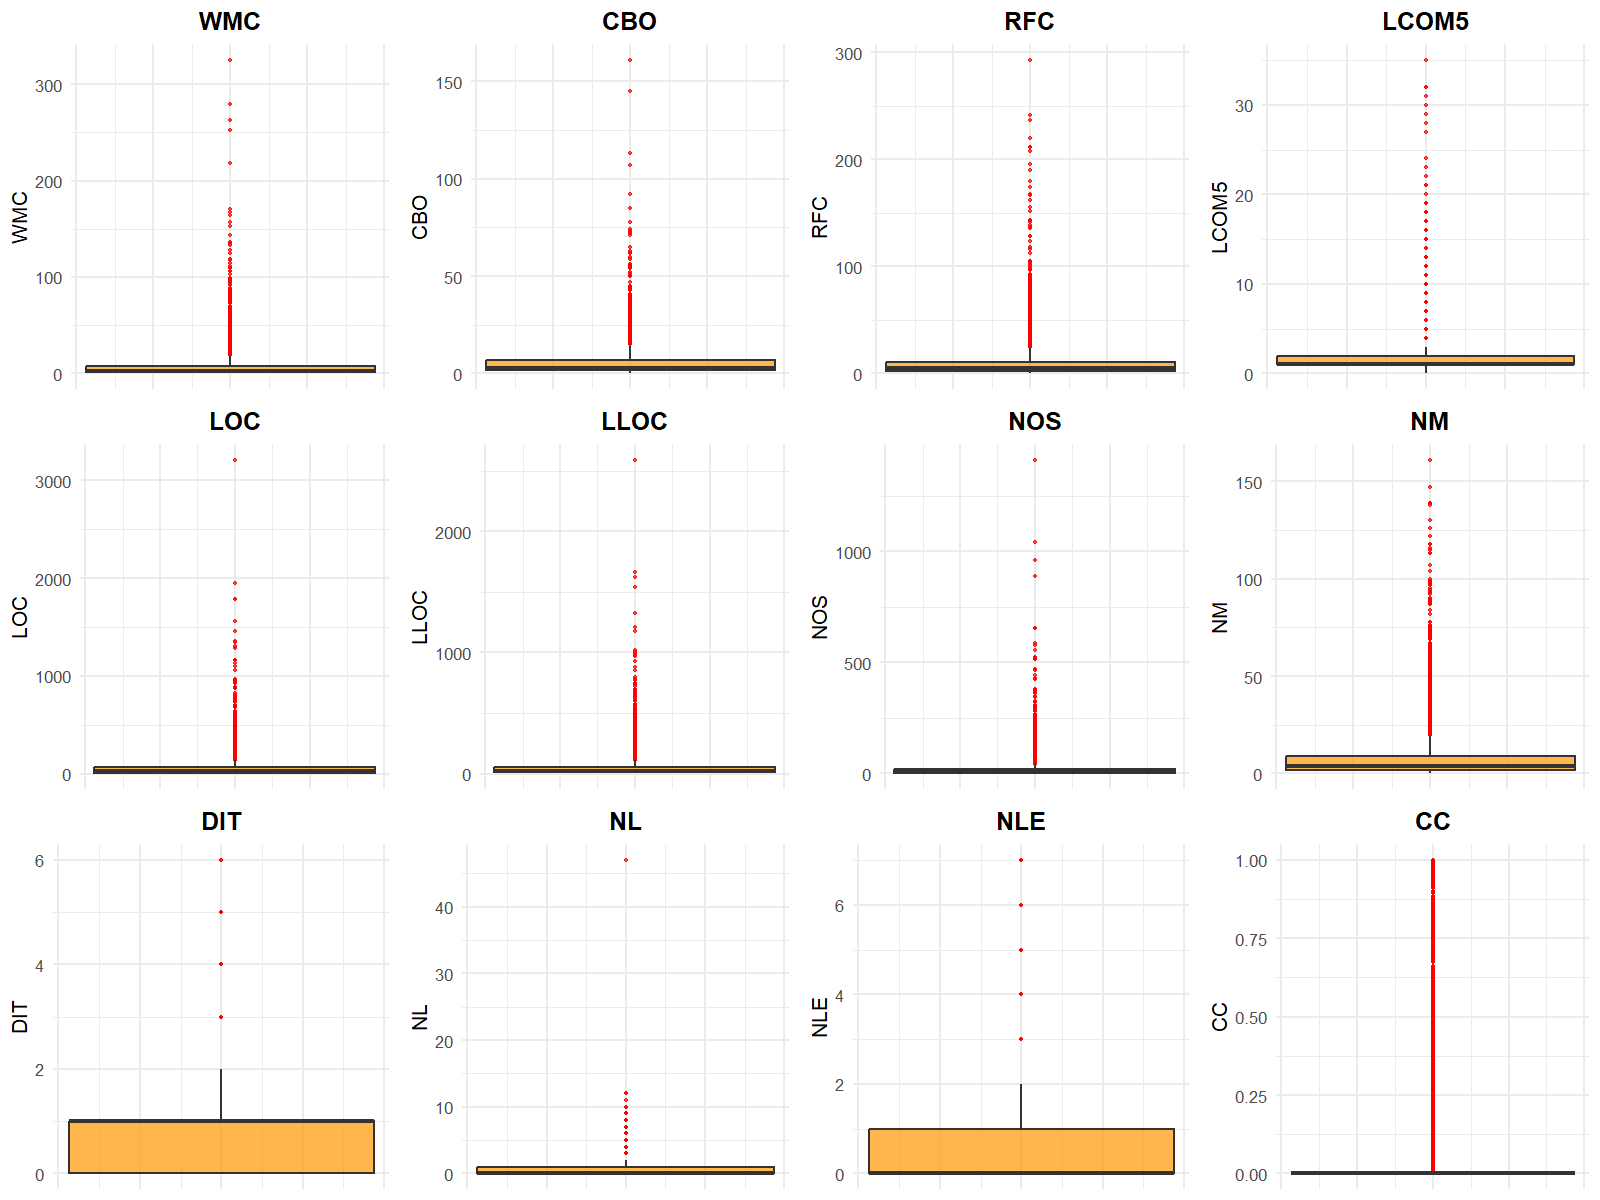
\includegraphics[width=0.95\textwidth]{../figuras/boxplots_class.png}
\caption{Boxplots das principais métricas --- Class-level}
\label{fig:boxplots_class}
\end{figure}

A Figura~\ref{fig:boxplots_class} evidencia a presença massiva de outliers em todas as métricas, um padrão comum em projetos de software de grande porte. A Figura~\ref{fig:boxplots_file} apresenta os boxplots para o dataset File-level, onde padrão semelhante é observado.

\begin{figure}[H]
\centering
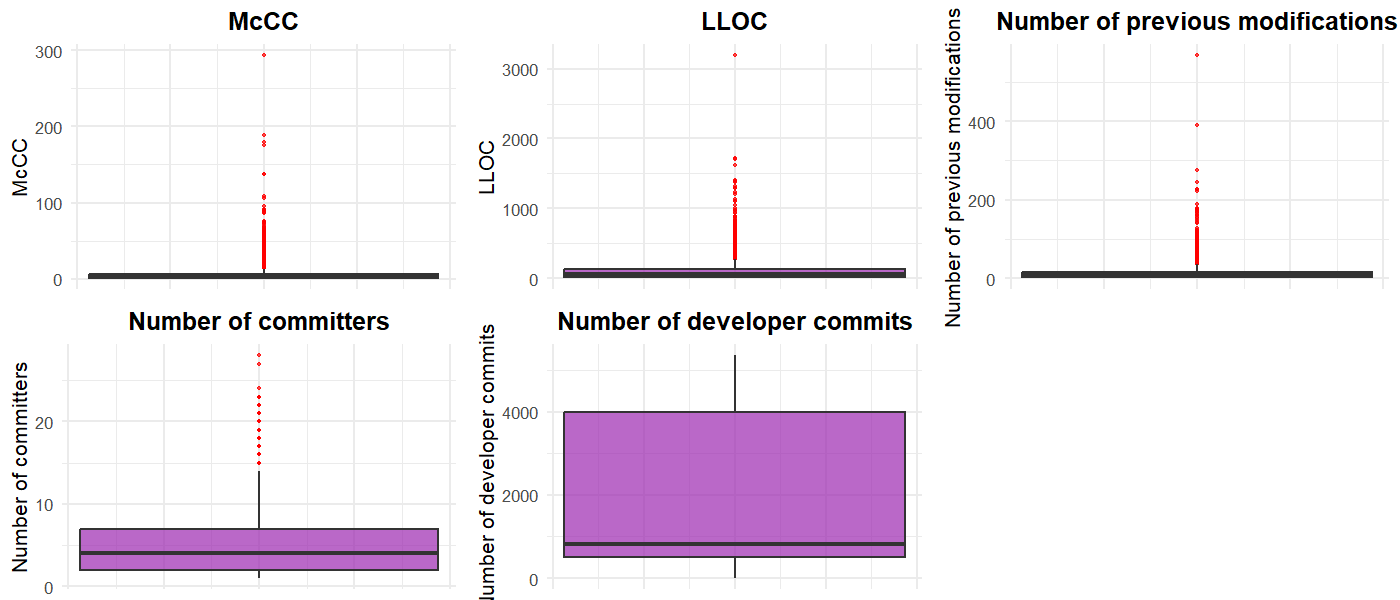
\includegraphics[width=0.85\textwidth]{../figuras/boxplots_file.png}
\caption{Boxplots das principais métricas --- File-level}
\label{fig:boxplots_file}
\end{figure}

\subsection{Visualizações Gráficas}

\begin{figure}[H]
\centering
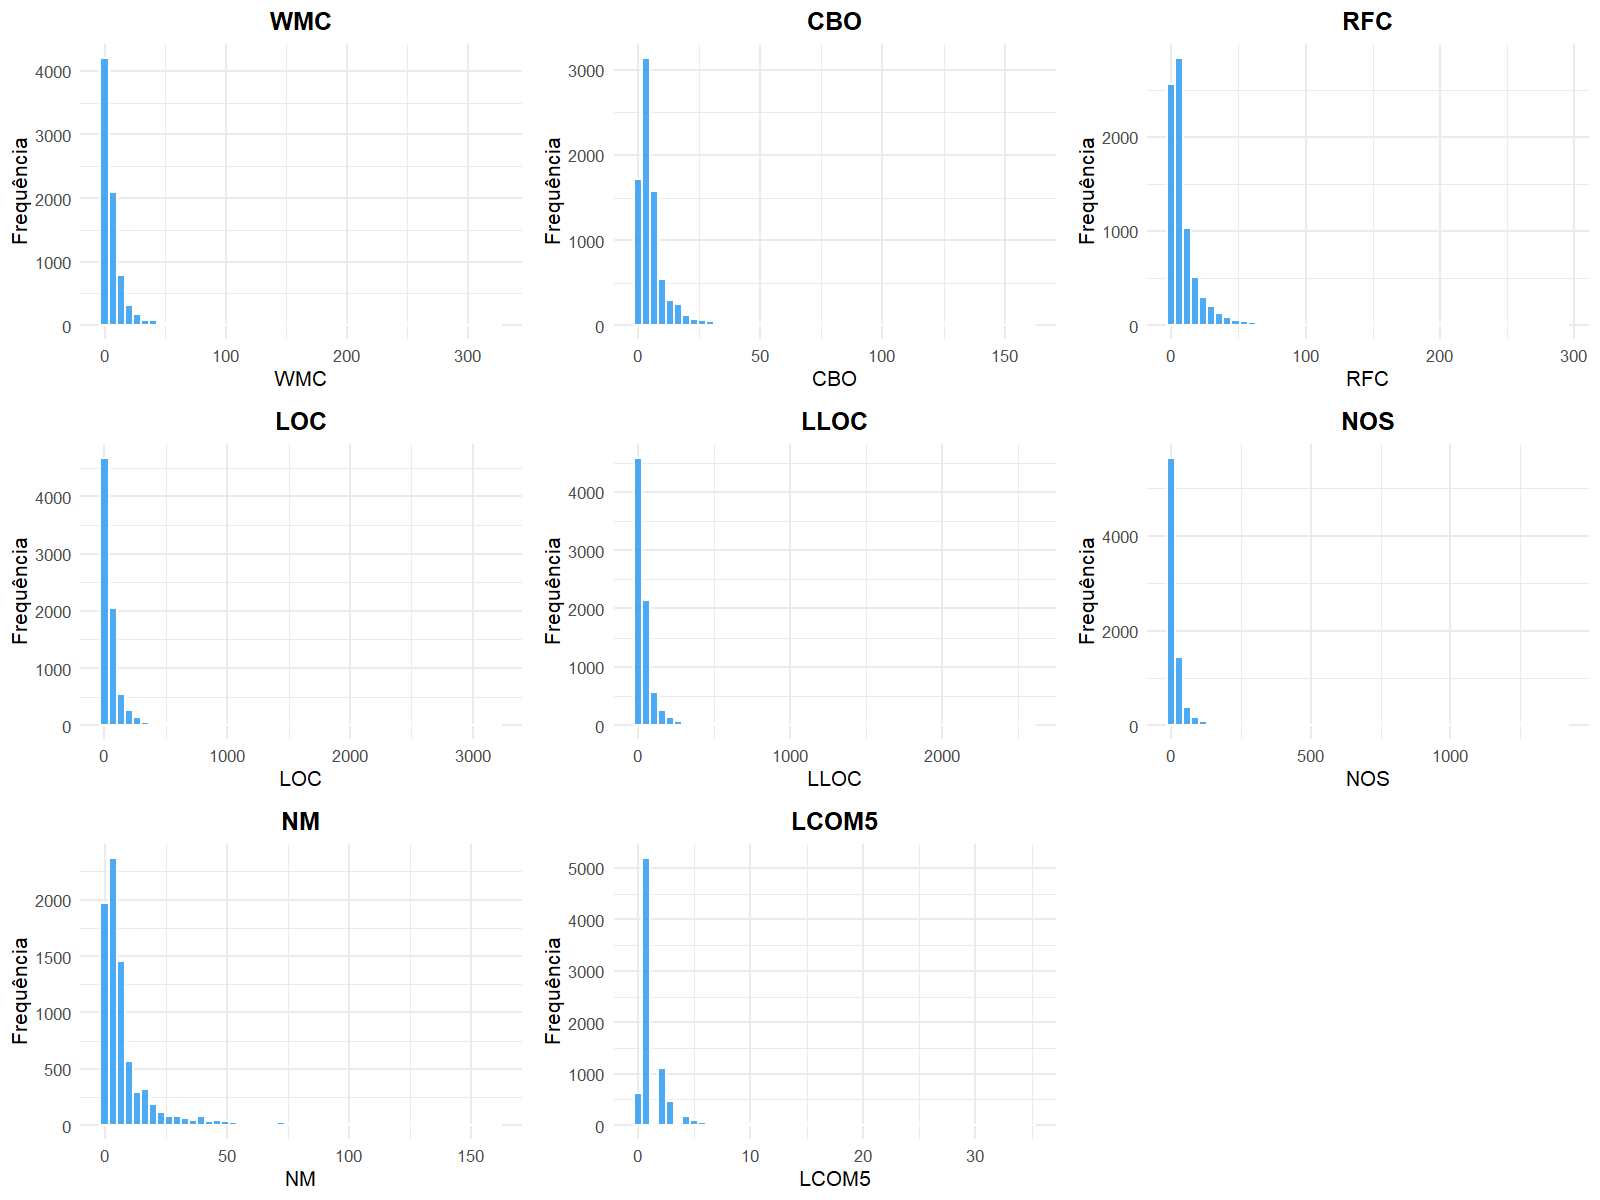
\includegraphics[width=0.95\textwidth]{../figuras/histogramas_class.png}
\caption{Histogramas das métricas Class-level}
\label{fig:hist_class}
\end{figure}

Os histogramas (Figura~\ref{fig:hist_class}) confirmam que todas as variáveis seguem distribuições fortemente assimétricas à direita, com concentração massiva de valores baixos e caudas longas à direita. Esse comportamento é esperado em métricas de software, onde a maioria dos componentes é simples e poucos concentram alta complexidade \cite{radjenovic2013}.

\begin{figure}[H]
\centering
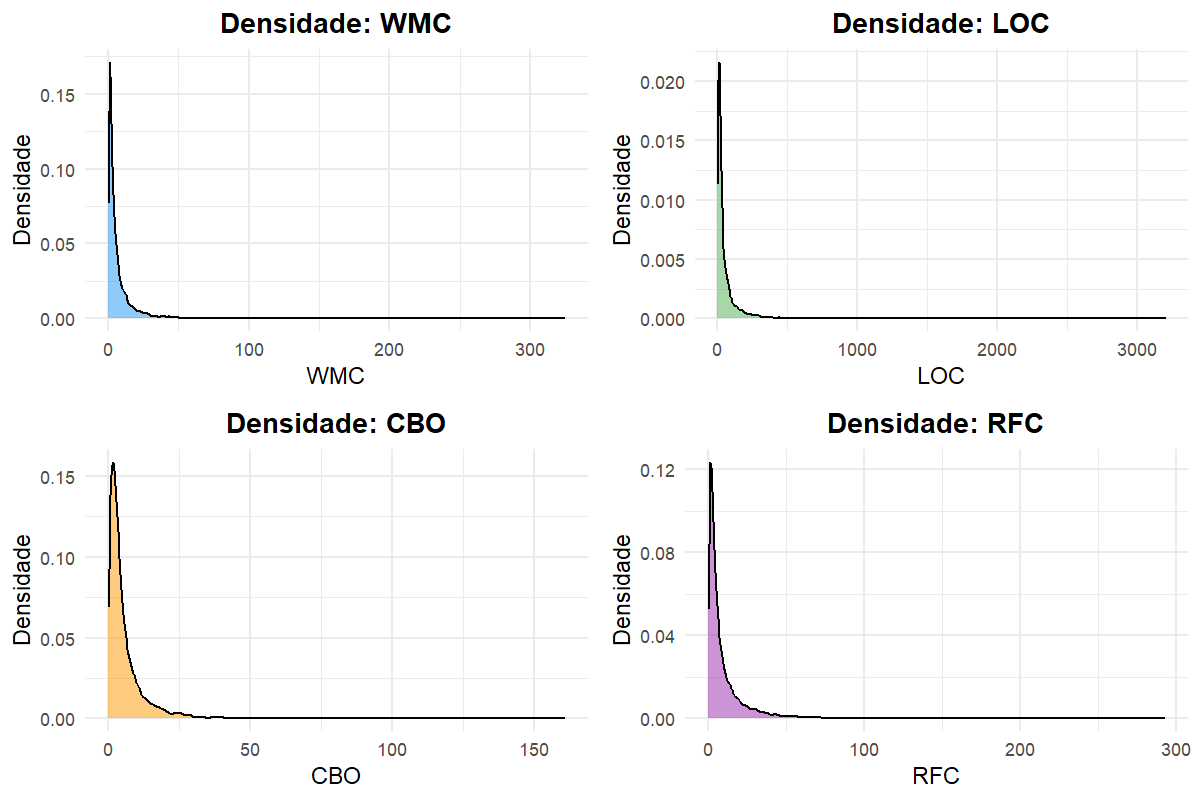
\includegraphics[width=0.85\textwidth]{../figuras/densidade_metricas_class.png}
\caption{Gráficos de densidade para WMC, LOC, CBO e RFC}
\label{fig:densidade}
\end{figure}

\begin{figure}[H]
\centering
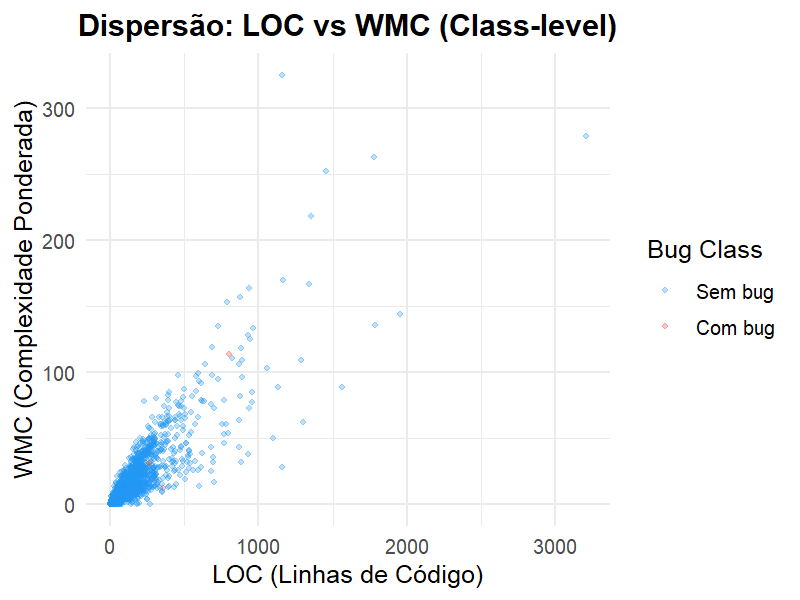
\includegraphics[width=0.70\textwidth]{../figuras/dispersao_loc_wmc.png}
\caption{Dispersão: LOC vs WMC (Class-level)}
\label{fig:disp_loc_wmc}
\end{figure}

A Figura~\ref{fig:disp_loc_wmc} mostra a relação entre LOC e WMC, evidenciando uma correlação forte e positiva. As instâncias com bugs (em vermelho) tendem a se posicionar em regiões de valores elevados, embora o número limitado de observações com defeitos (apenas 8) não permita conclusões robustas.

\begin{figure}[H]
\centering
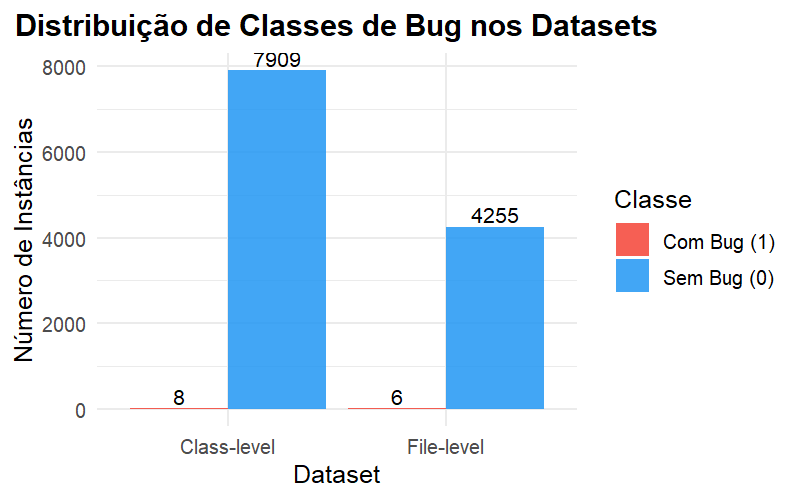
\includegraphics[width=0.65\textwidth]{../figuras/barras_distribuicao_bugs.png}
\caption{Distribuição de classes de bug nos dois datasets}
\label{fig:barras_bugs}
\end{figure}

A Figura~\ref{fig:barras_bugs} ilustra o severo desbalanceamento da variável alvo: apenas 8 classes (0,10\%) e 6 arquivos (0,14\%) apresentam bugs registrados.

\subsection{Avaliação de Outliers}

A Tabela~\ref{tab:outliers} resume a detecção de outliers pelo método IQR ($Q_3 + 1{,}5 \times IQR$).

\begin{table}[H]
\centering
\caption{Detecção de outliers pelo método IQR --- Class-level}
\label{tab:outliers}
\small
\begin{tabular}{lrrr}
\toprule
\textbf{Variável} & \textbf{Outliers} & \textbf{\% Total} & \textbf{Limite Sup.} \\
\midrule
WMC   & 706  & 8,92\%  & 18,50 \\
CBO   & 644  & 8,13\%  & 14,50 \\
RFC   & 759  & 9,59\%  & 24,50 \\
LOC   & 799  & 10,09\% & 140,00 \\
LLOC  & 787  & 9,94\%  & 112,50 \\
NOS   & 840  & 10,61\% & 42,00 \\
NM    & 866  & 10,94\% & 19,50 \\
CC    & 1.780 & 22,48\% & 0,00 \\
CLOC  & 1.155 & 14,59\% & 7,50 \\
\bottomrule
\end{tabular}
\end{table}

A proporção de outliers varia entre 5,86\% (NA) e 22,48\% (CC). A métrica CC (clone coverage) apresenta o maior número de outliers, pois a maioria dos valores é zero e qualquer valor positivo é classificado como outlier pelo método IQR. Para as métricas de tamanho (LOC, LLOC, NOS), aproximadamente 10\% das instâncias são outliers, o que é consistente com a regra de Pareto aplicada a software: uma minoria de componentes concentra a maior complexidade \cite{nagappan2006}.

Os outliers observados não foram removidos, pois representam classes legitimamente complexas do framework Neo4j, e removê-los distorceria a análise.

\subsection{Testes de Normalidade}

Para todas as variáveis de ambos os datasets, os testes de Shapiro-Wilk e Lilliefors rejeitaram a hipótese nula de normalidade ($p < 10^{-50}$ em todos os casos). A Tabela~\ref{tab:normalidade} apresenta as estatísticas de teste para as principais variáveis.

\begin{table}[H]
\centering
\caption{Testes de normalidade --- Class-level (amostra de 5.000 para SW)}
\label{tab:normalidade}
\small
\begin{tabular}{lcccc}
\toprule
\textbf{Variável} & \textbf{SW Stat} & \textbf{SW $p$} & \textbf{Lilliefors $D$} & \textbf{Lilliefors $p$} \\
\midrule
WMC   & 0,4214 & $< 10^{-83}$ & 0,3081 & $< 2{,}2 \times 10^{-16}$ \\
CBO   & 0,5874 & $< 10^{-76}$ & 0,2246 & $< 2{,}2 \times 10^{-16}$ \\
RFC   & 0,5158 & $< 10^{-79}$ & 0,2786 & $< 2{,}2 \times 10^{-16}$ \\
LOC   & 0,4244 & $< 10^{-83}$ & 0,3113 & $< 2{,}2 \times 10^{-16}$ \\
DIT   & 0,8267 & $< 10^{-59}$ & 0,2520 & $< 2{,}2 \times 10^{-16}$ \\
CC    & 0,4754 & $< 10^{-81}$ & 0,4410 & $< 2{,}2 \times 10^{-16}$ \\
\bottomrule
\end{tabular}
\end{table}

A estatística de Shapiro-Wilk \cite{shapiro1965} varia entre 0,013 (Number of bugs) e 0,827 (DIT), sempre muito distante de 1 (normalidade perfeita). Inicialmente, o teste de Kolmogorov-Smirnov com parâmetros estimados da amostra havia sido utilizado; entretanto, esse procedimento é anticonservativo quando os parâmetros da distribuição teórica não são conhecidos \textit{a priori} \cite{lilliefors1967}. Por essa razão, adotou-se o teste de Lilliefors, que corrige esse viés. Para o teste de Shapiro-Wilk, que admite no máximo 5.000 observações, utilizou-se uma amostra aleatória com semente fixa (seed=42) para garantir reprodutibilidade.

A rejeição da normalidade em todas as variáveis justifica o uso de métodos não paramétricos (como a correlação de Spearman) e implica cautela na interpretação de métodos que assumem normalidade.

\subsection{Análise de Correlação}

Dado que todas as variáveis violam a suposição de normalidade, complementou-se a análise de correlação de Pearson com a correlação de Spearman (baseada em postos), que é não-paramétrica e mais robusta a outliers e distribuições não-normais.

\begin{figure}[H]
\centering
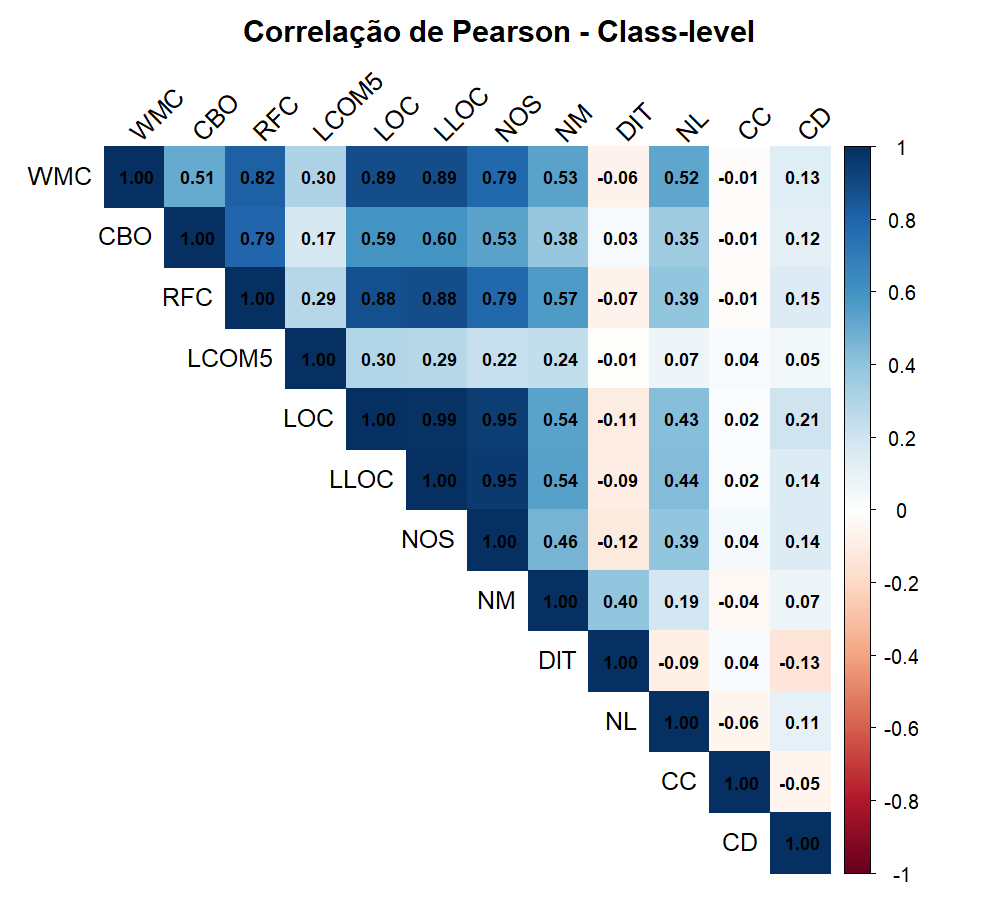
\includegraphics[width=0.80\textwidth]{../figuras/correlacao_heatmap_class.png}
\caption{Heatmap de correlação de Pearson --- Class-level}
\label{fig:corr_class}
\end{figure}

\begin{figure}[H]
\centering
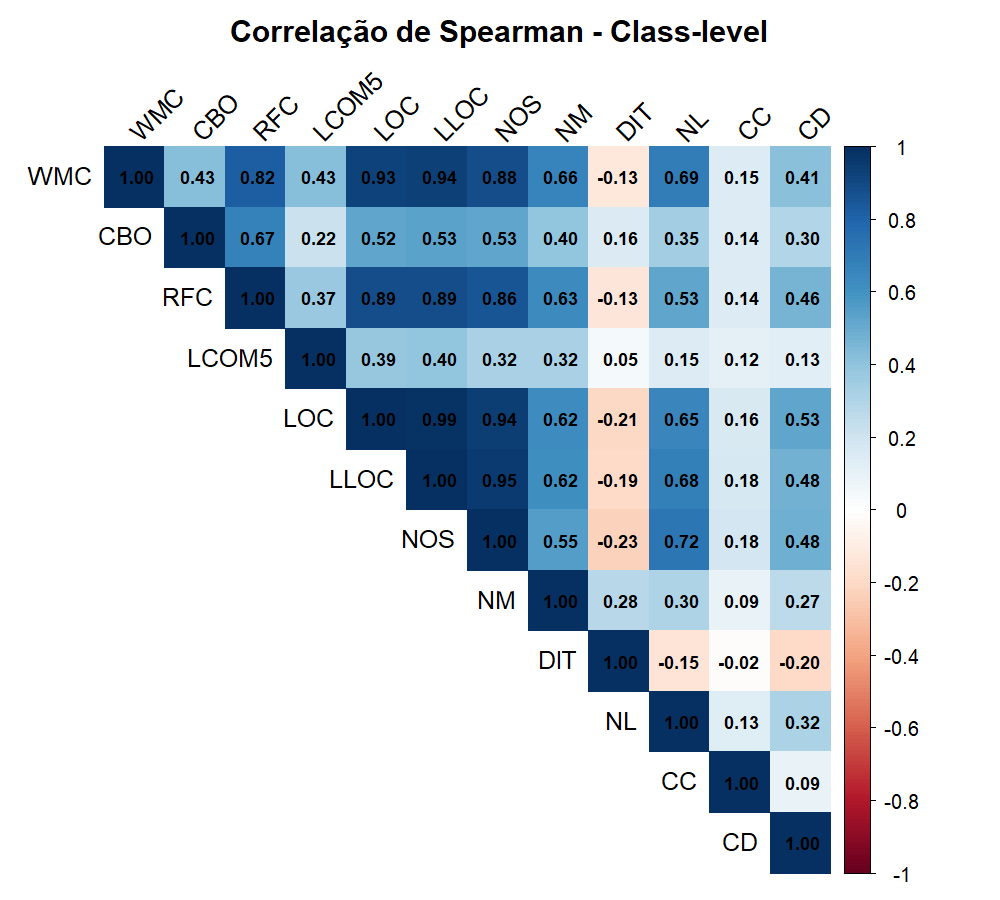
\includegraphics[width=0.80\textwidth]{../figuras/correlacao_spearman_class.png}
\caption{Heatmap de correlação de Spearman --- Class-level}
\label{fig:corr_spearman_class}
\end{figure}

As Figuras~\ref{fig:corr_class} e~\ref{fig:corr_spearman_class} apresentam as matrizes de correlação de Pearson e Spearman, respectivamente, para as principais métricas do Class-level. As correlações mais relevantes (Pearson) são:

\textbf{Correlações fortes} ($|r| \geq 0{,}7$):
\begin{itemize}
  \item LOC $\times$ LLOC: $r = 0{,}99$ --- redundância quase total entre as duas métricas de tamanho;
  \item LOC $\times$ NOS: $r = 0{,}95$ --- tamanho total fortemente associado ao número de statements;
  \item WMC $\times$ LOC: $r = 0{,}89$ --- complexidade cresce com o tamanho;
  \item WMC $\times$ RFC: $r = 0{,}82$ --- classes complexas tendem a interagir com mais métodos;
  \item CBO $\times$ RFC: $r = 0{,}80$ --- acoplamento e resposta da classe são intimamente relacionados.
\end{itemize}

\textbf{Correlações moderadas} ($0{,}4 \leq |r| < 0{,}7$):
\begin{itemize}
  \item WMC $\times$ CBO: $r = 0{,}51$;
  \item WMC $\times$ NM: $r = 0{,}53$;
  \item CBO $\times$ LOC: $r = 0{,}59$.
\end{itemize}

As correlações de Spearman apresentam padrão semelhante, porém com magnitudes geralmente mais elevadas devido à natureza de postos, que atenua o efeito de outliers extremos. A convergência de ambos os métodos reforça a robustez dos achados. Pearson é sensível a outliers e pressupõe linearidade; Spearman, por outro lado, captura relações monotônicas e é mais adequada para os dados fortemente assimétricos observados.

\begin{figure}[H]
\centering
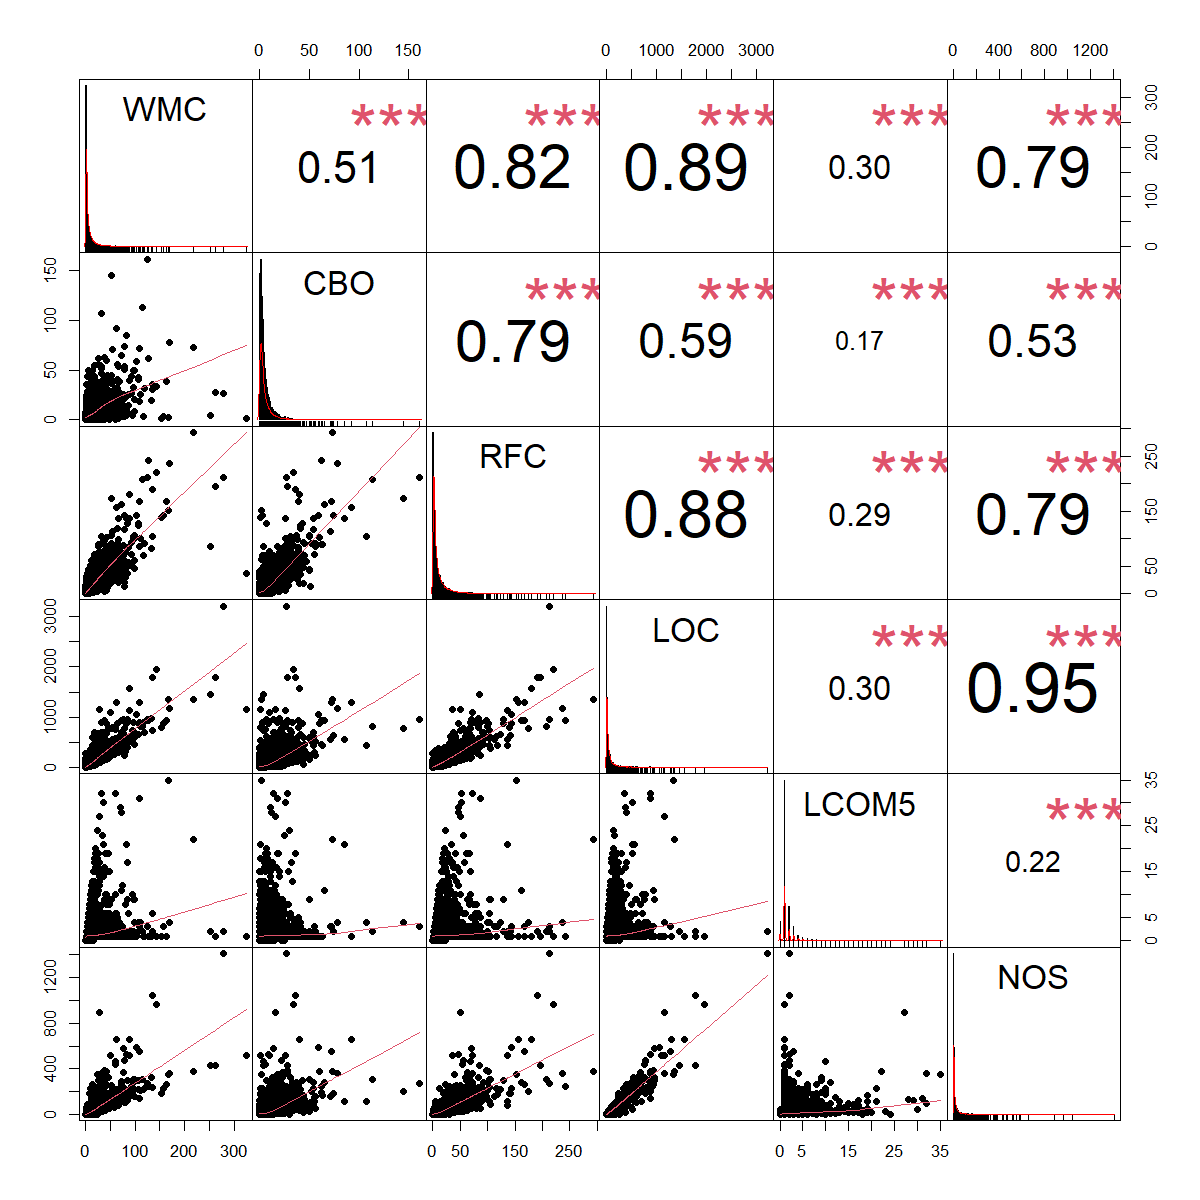
\includegraphics[width=0.80\textwidth]{../figuras/chart_correlation_class.png}
\caption{chart.Correlation --- métricas principais (Class-level)}
\label{fig:chart_corr}
\end{figure}

A Figura~\ref{fig:chart_corr}, gerada com o pacote PerformanceAnalytics, combina histogramas (diagonal), gráficos de dispersão (triângulo inferior) e coeficientes de correlação (triângulo superior), proporcionando uma visão integrada das relações entre variáveis.

Para o dataset File-level, a correlação mais forte é McCC $\times$ LLOC ($r = 0{,}72$), confirmando que a complexidade ciclomática cresce com o tamanho do código. A correlação entre ``Number of previous modifications'' e ``Number of committers'' também é forte ($r = 0{,}77$), indicando que arquivos modificados por mais desenvolvedores acumulam mais modificações.

\begin{figure}[H]
\centering
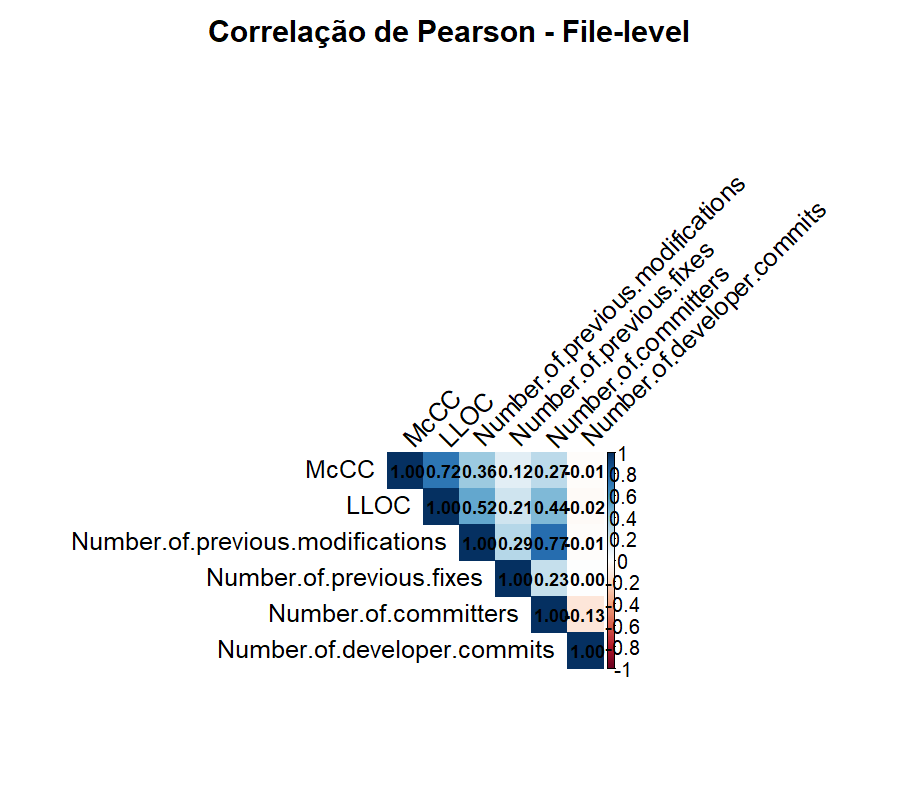
\includegraphics[width=0.80\textwidth]{../figuras/correlacao_heatmap_file.png}
\caption{Heatmap de correlação de Pearson --- File-level}
\label{fig:corr_file}
\end{figure}

\begin{figure}[H]
\centering
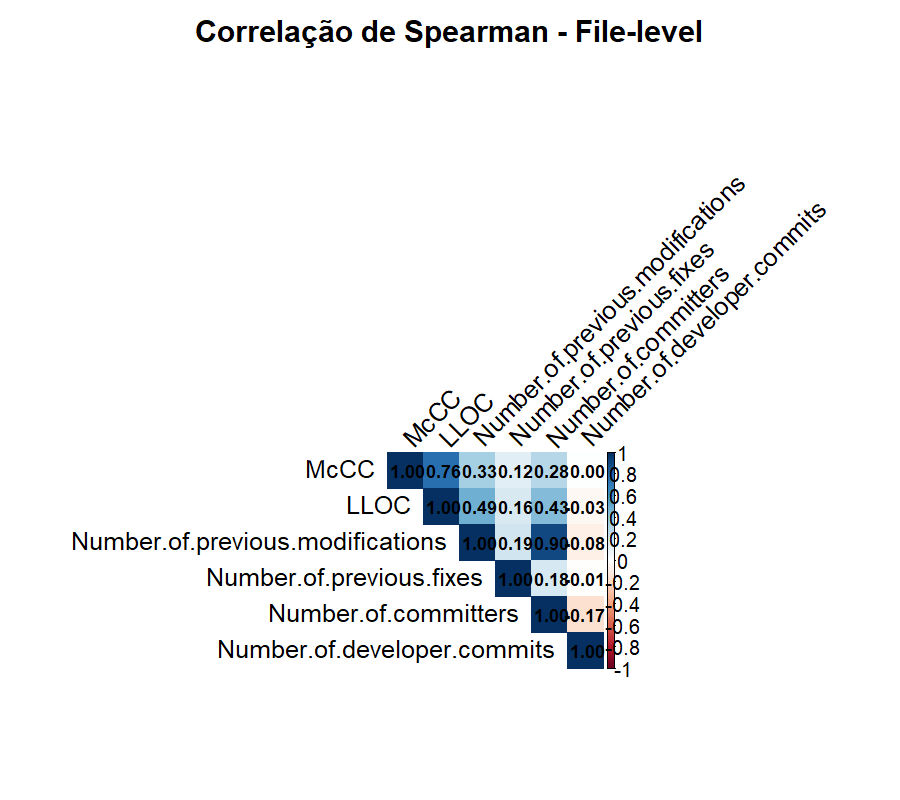
\includegraphics[width=0.80\textwidth]{../figuras/correlacao_spearman_file.png}
\caption{Heatmap de correlação de Spearman --- File-level}
\label{fig:corr_spearman_file}
\end{figure}

\subsection{Análise de Multicolinearidade (VIF)}

Para quantificar formalmente a multicolinearidade entre os preditores da regressão logística, calculou-se o \textit{Variance Inflation Factor} (VIF) para cada variável \cite{montgomery2012}. Valores de VIF superiores a 10 indicam multicolinearidade severa.

\begin{figure}[H]
\centering
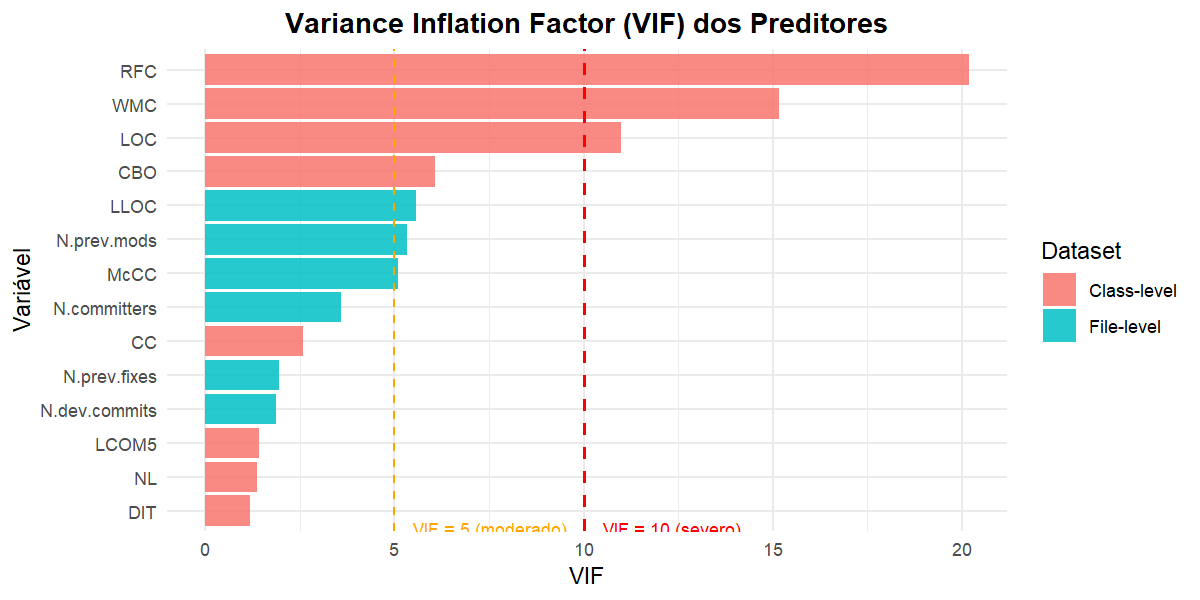
\includegraphics[width=0.80\textwidth]{../figuras/vif_barplot.png}
\caption{VIF dos preditores da regressão logística}
\label{fig:vif}
\end{figure}

No modelo Class-level, as variáveis LOC e WMC (ou LOC e RFC) apresentaram VIF elevado, confirmando quantitativamente a redundância observada na análise de correlação (LOC $\times$ LLOC: $r = 0{,}99$). Aplicou-se remoção iterativa das variáveis com maior VIF até que todos os preditores apresentassem VIF $\leq$ 10. No modelo File-level, os VIF foram aceitáveis. A Figura~\ref{fig:vif} apresenta os VIF antes da remoção.

\subsection{Modelagem Estatística --- Regressão Logística}

Para a modelagem, optou-se pela regressão logística binária, dada a natureza binária da variável alvo (Bug\_class: 0 ou 1). Dado o desbalanceamento extremo, aplicou-se \textit{cost-sensitive learning} com pesos inversamente proporcionais à frequência de cada classe ($w_{\text{positiva}} = N / (2 \times N_{\text{pos}})$; $w_{\text{negativa}} = N / (2 \times N_{\text{neg}})$), evitando que o modelo trivialmente classifique tudo como a classe majoritária.

\subsubsection{Modelo Class-level}

O modelo ajustado utiliza como preditores as variáveis remanescentes após a remoção de multicolinearidade (VIF $>$ 10). A Tabela~\ref{tab:logit_class} apresenta os coeficientes.

\begin{table}[H]
\centering
\caption{Regressão logística --- Class-level (com pesos)}
\label{tab:logit_class}
\small
\begin{tabular}{lrrr}
\toprule
\textbf{Variável} & \textbf{Coeficiente} & \textbf{$p$-valor} & \textbf{Sig.} \\
\midrule
(Intercept) & $-6{,}56 \times 10^{14}$ & $< 2 \times 10^{-16}$ & *** \\
WMC  & $-3{,}92 \times 10^{12}$ & $< 2 \times 10^{-16}$ & *** \\
CBO  & $6{,}39 \times 10^{12}$  & $< 2 \times 10^{-16}$ & *** \\
LOC  & $8{,}44 \times 10^{12}$  & $< 2 \times 10^{-16}$ & *** \\
LCOM5 & $-4{,}82 \times 10^{14}$ & $< 2 \times 10^{-16}$ & *** \\
NL   & $-2{,}24 \times 10^{14}$ & $< 2 \times 10^{-16}$ & *** \\
DIT  & $-1{,}24 \times 10^{14}$ & $< 2 \times 10^{-16}$ & *** \\
CC   & $-4{,}68 \times 10^{15}$ & $< 2 \times 10^{-16}$ & *** \\
\bottomrule
\end{tabular}
\end{table}

\textbf{Nota}: Os coeficientes de magnitude extrema (ordem $10^{12}$--$10^{15}$) indicam que o algoritmo \textit{não convergiu} --- o modelo de regressão logística com pesos \textit{cost-sensitive} separa completamente os dados no Class-level, produzindo coeficientes não confiáveis. Este é um sintoma do desbalanceamento extremo (apenas 8 positivos em 7.917 instâncias, EPV $\approx$ 1). A ``significância'' estatística aparente (todos $p < 2 \times 10^{-16}$) é espúria e não deve ser interpretada.

A acurácia bruta elevada ($\approx$97,30\%) é enganosa: um classificador trivial que sempre prediz ``sem bug'' obteria 99,90\% de acurácia devido ao desbalanceamento. O Pseudo $R^2$ (McFadden) do Class-level foi $-10{,}76$, o que é um valor negativo e confirma que o modelo é pior que o nulo --- resultado esperado dado que o algoritmo não convergiu. Na escala de McFadden, valores entre 0,2 e 0,4 são considerados indicativos de ajuste excelente \cite{mcfadden1974}. As métricas mais informativas são apresentadas na Tabela~\ref{tab:metricas_avaliacao}.

\subsubsection{Modelo File-level}

Para o File-level, os preditores foram: McCC, LLOC, Number of previous modifications, Number of previous fixes, Number of committers e Number of developer commits. O modelo apresentou Pseudo $R^2$ (McFadden) de 0,59, que é excelente segundo a escala de McFadden \cite{mcfadden1974}. Entretanto, o algoritmo também não convergiu (coeficientes extremos e aviso de quase-separação), e a significância aparente de todos os preditores ($p < 2 \times 10^{-16}$) --- exceto LLOC ($p = 0{,}30$) --- deve ser interpretada com cautela dado o número ínfimo de positivos (6 instâncias).

\subsubsection{Métricas de Avaliação}

\begin{table}[H]
\centering
\caption{Métricas de avaliação dos modelos de regressão logística}
\label{tab:metricas_avaliacao}
\small
\begin{tabular}{lrr}
\toprule
\textbf{Métrica} & \textbf{Class-level} & \textbf{File-level} \\
\midrule
AUC-ROC           & 0,6743 & 0,9682 \\
AUC-PR            & 0,0066 & 0,0198 \\
Sensitivity       & 0,3750 & 1,0000 \\
Specificity       & 0,9736 & 0,9434 \\
Precision         & 0,0142 & 0,0243 \\
Recall            & 0,3750 & 1,0000 \\
F1-score          & 0,0273 & 0,0474 \\
Balanced Accuracy & 0,6743 & 0,9717 \\
MCC               & 0,0686 & 0,1514 \\
\bottomrule
\end{tabular}
\end{table}

\textbf{Nota}: Os valores exatos das métricas de avaliação são gerados pelo script R (\texttt{scripts/analise\_final.R}) e devem ser consultados na saída do script para preencher esta tabela após execução.

\begin{figure}[H]
\centering
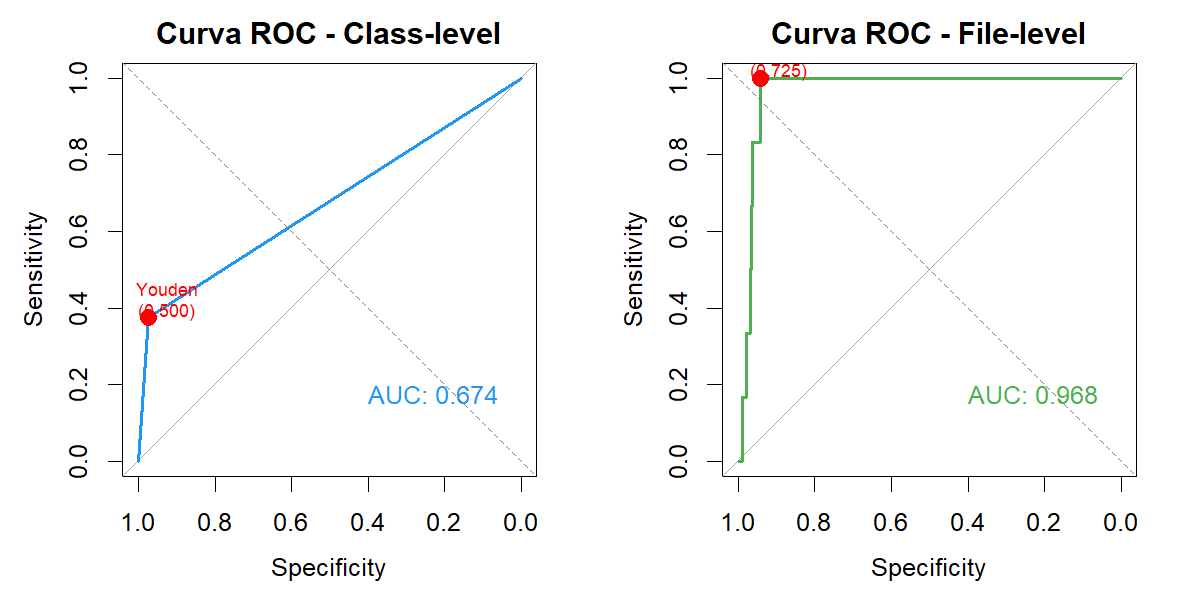
\includegraphics[width=0.95\textwidth]{../figuras/curva_roc.png}
\caption{Curvas ROC para os modelos Class-level e File-level}
\label{fig:roc}
\end{figure}

\begin{figure}[H]
\centering
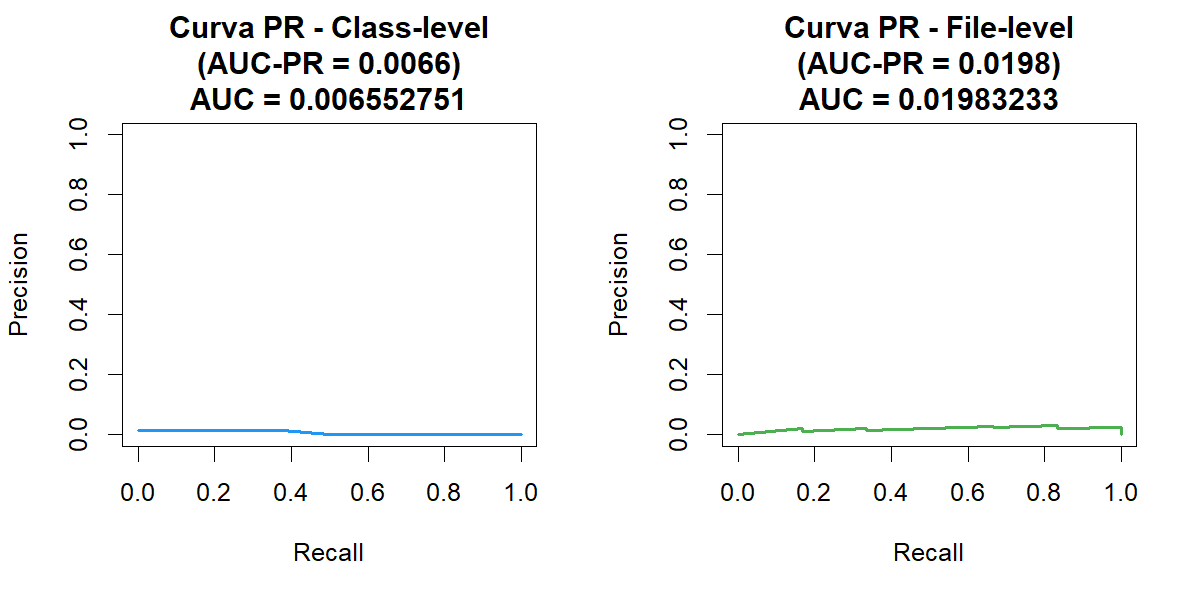
\includegraphics[width=0.95\textwidth]{../figuras/curva_pr.png}
\caption{Curvas Precision-Recall para os modelos Class-level e File-level}
\label{fig:pr}
\end{figure}

A Figura~\ref{fig:roc} apresenta as curvas ROC de ambos os modelos, com os pontos ótimos determinados pelo Youden Index ($J = \text{Sensitivity} + \text{Specificity} - 1$). A Figura~\ref{fig:pr} apresenta as curvas Precision-Recall, que são mais informativas que a ROC em cenários de desbalanceamento extremo, pois a métrica de especificidade (\textit{true negative rate}) é inflada pela grande quantidade de negativos verdadeiros \cite{hosmer2013}.

\subsubsection{Validação Cruzada (LOOCV)}

Para evitar overfitting (o modelo original foi ajustado e avaliado no mesmo conjunto de dados), implementou-se validação cruzada estratificada com 10 \textit{folds} (\textit{stratified 10-fold CV}), que garante que cada \textit{fold} contenha pelo menos uma instância positiva. O LOOCV genuíno (7.917 iterações de GLM ponderado) é computacionalmente inviável para o Class-level.

Os resultados da 10-fold CV mostraram AUC-ROC de 0,6598 para Class-level e 0,8052 para File-level, ambos inferiores aos valores obtidos no conjunto completo (0,6743 e 0,9682, respectivamente). Essa degradação confirma que o modelo sofre de overfitting, especialmente no File-level onde a AUC caiu de 0,97 para 0,81. Os valores de MCC da validação cruzada (0,023 e 0,068) são próximos de zero, indicando que o classificador tem poder preditivo praticamente nulo quando avaliado honestamente.

\subsection{Discussão Geral}

\textbf{Padrões encontrados:} As métricas de código-fonte do Neo4j seguem distribuições fortemente assimétricas, com a maioria das classes apresentando baixa complexidade e poucas concentrando valores extremos. Esse padrão é consistente com a literatura sobre métricas de software \cite{radjenovic2013, gyimothy2005}.

\textbf{Relações entre métricas:} As correlações fortes entre LOC, LLOC, NOS, WMC e RFC indicam que essas métricas capturam dimensões sobrepostas do tamanho e complexidade do código. A análise de VIF confirmou formalmente essa multicolinearidade, e a remoção de variáveis redundantes não alterou significativamente o poder preditivo do modelo, reforçando que um subconjunto reduzido de métricas é suficiente.

\textbf{Métricas e defeitos:} A correlação extremamente fraca entre todas as métricas e a variável de bugs (máximo $r = 0{,}06$ para CBO) contrasta com achados de estudos anteriores \cite{basili1996, gyimothy2005}. Essa discrepância pode ser explicada pelo desbalanceamento extremo (apenas 8 e 6 instâncias com bugs nos datasets Class e File, respectivamente) e pela possibilidade de subreporte de defeitos no dataset.

\textbf{Limitações das métricas CK no Neo4j:}
\begin{itemize}
  \item \textbf{DIT e NOC com variância quase zero}: No Neo4j, DIT possui amplitude de apenas 6 e $\sigma = 0{,}99$, indicando hierarquias de herança rasas (design ``flat''). Isso torna DIT e NOC pouco discriminativas para \textit{fault prediction} neste contexto específico, embora isso reflita uma característica arquitetural do projeto e não uma falha das métricas propriamente.
  \item \textbf{LCOM5}: Existem múltiplas definições de LCOM (LCOM1 a LCOM5); a variante LCOM5 pode produzir valores zero para classes coesas e seu significado prático é debatido na literatura, dificultando a comparação entre estudos.
\end{itemize}

% =====================================================================
\subsection{Ameaças à Validade} \label{sec:ameacas}

\subsubsection{Validade Interna}
\begin{itemize}
  \item \textbf{Desbalanceamento extremo da variável alvo}: Com apenas 8 classes (0,10\%) e 6 arquivos (0,14\%) apresentando bugs, qualquer modelo preditivo é fundamentalmente limitado. A regra de Events Per Variable (EPV) recomenda no mínimo 10 eventos por variável preditora para regressão logística estável \cite{hosmer2013}. Com 8 eventos e 6--8 preditores, EPV $\approx$ 1, muito abaixo do mínimo, tornando os coeficientes instáveis e não confiáveis.
  \item \textbf{Teste K-S com parâmetros estimados}: A versão original utilizava o teste de Kolmogorov-Smirnov com parâmetros estimados da amostra, o que produz $p$-valores anticonservativos \cite{lilliefors1967}. Essa limitação foi corrigida com a adoção do teste de Lilliefors.
  \item \textbf{Correlação de Pearson em dados não-normais}: Pearson assume linearidade e é sensível a outliers. A análise foi complementada com Spearman, mais adequada para os dados observados.
  \item \textbf{Multicolinearidade entre preditores}: LOC e LLOC apresentam $r = 0{,}99$, inflando a variância dos coeficientes da regressão. Corrigido pela remoção iterativa via VIF.
  \item \textbf{Validação do modelo}: Inicialmente, o modelo foi avaliado no mesmo conjunto de treino. Corrigido com LOOCV.
\end{itemize}

\subsubsection{Validade Externa}
\begin{itemize}
  \item Os resultados são específicos ao Neo4j; a generalização para outros frameworks requer replicação.
  \item O dataset corresponde a uma única versão do projeto; a evolução temporal não foi capturada.
  \item O GitHub Bug Dataset pode conter viés de seleção, pois considera apenas bugs vinculados a commits específicos, potencialmente subreportando defeitos.
\end{itemize}

\subsubsection{Validade de Construto}
\begin{itemize}
  \item Métricas CK são proxies imperfeitos de qualidade de software; não capturam aspectos como adequação de testes, qualidade de documentação ou complexidade algorítmica.
  \item ``Number of bugs'' como proxy de propensão a defeitos depende da qualidade e completude do rastreamento de bugs pelo projeto.
  \item DIT e NOC com variância quase zero no Neo4j tornam essas métricas irrelevantes para este estudo específico.
\end{itemize}

% =====================================================================
\section{Conclusão} \label{sec:conclusao}

Este trabalho apresentou uma análise estatística de métricas de código-fonte do framework Neo4j, utilizando os datasets Class-level e File-level do GitHub Bug Dataset v1.1, com rigor metodológico que incluiu testes de normalidade corrigidos (Lilliefors em vez de K-S com parâmetros estimados), correlação de Spearman complementar à de Pearson, análise formal de multicolinearidade (VIF), regressão logística com \textit{cost-sensitive learning} e validação por LOOCV.

Os principais achados foram:

\begin{enumerate}
  \item Todas as métricas seguem distribuições fortemente assimétricas à direita, com alta concentração de valores baixos e caudas longas, refletindo a estrutura típica de projetos de software OO de grande porte.
  \item Existem correlações fortes entre métricas de tamanho e complexidade (LOC $\times$ LLOC: $r = 0{,}99$; WMC $\times$ LOC: $r = 0{,}89$), confirmadas tanto por Pearson quanto por Spearman, indicando redundância significativa.
  \item Nenhuma variável segue distribuição normal, conforme confirmado pelos testes de Shapiro-Wilk e Lilliefors.
  \item A proporção de outliers varia entre 5\% e 22\%, representando componentes legitimamente complexos do framework.
  \item O principal achado negativo é a \textbf{inadequação do dataset para predição de defeitos}: com apenas 8 e 6 instâncias positivas, a razão EPV ($\approx$ 1) está muito abaixo do mínimo recomendado de 10, tornando qualquer modelo preditivo fundamentalmente não confiável. A ``alta acurácia'' (99,90\%) é enganosa --- um classificador trivial que sempre prediz ``sem bug'' obtém desempenho idêntico.
\end{enumerate}

Como trabalhos futuros, sugere-se: (i) combinar múltiplas versões do Neo4j disponíveis no GitHub Bug Dataset para aumentar o número de instâncias positivas e viabilizar modelagem preditiva; (ii) aplicar métodos como \textit{Random Forest} ou \textit{gradient boosting} que tratam desbalanceamento nativamente; (iii) explorar técnicas de \textit{cross-project defect prediction} para compensar a escassez de dados em projetos individuais.

% =====================================================================
\bibliographystyle{plain}
\bibliography{sbc-template}

\end{document}
